%----------Chương 3
\section*{CHƯƠNG 3 - TRIỂN KHAI HỆ THỐNG}
\addcontentsline{toc}{section}{\numberline{}CHƯƠNG 3 -  XÂY DỰNG HỆ THỐNG}
\setcounter{section}{3}
\setcounter{subsection}{0}
\setcounter{figure}{0}
\setcounter{table}{0}
	
%----------Phần trình bày nội dung chương 3

\subsection{ Mô hình thiết kế hệ thống:}
Mô hình mô phỏng hệ thống  một công ty với 2 chi nhánh sử dụng 3 Router và 3 Switch.

-Sơ đồ vật lý:

    \begin{figure}[h!] % Môi trường figure
        \centering % Căn giữa hình ảnh trong cột văn bản
        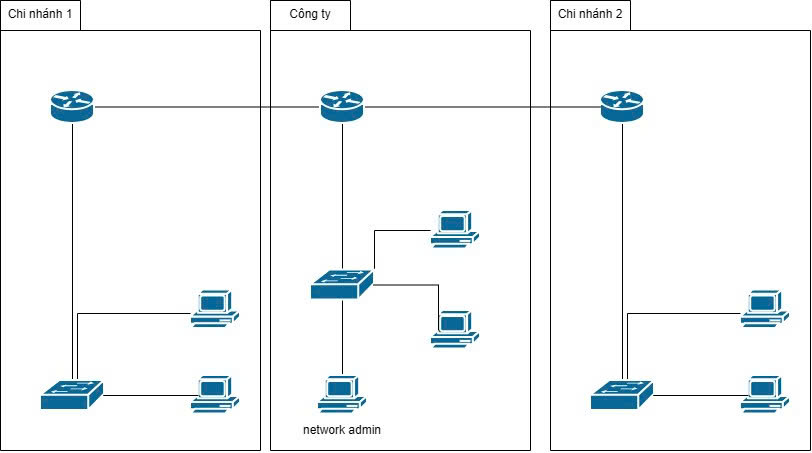
\includegraphics[width=0.7\textwidth]{image/so_do_vat_ly.jpg}
        % 

        \caption{Sơ đồ vật lý} % Chú thích hình ảnh
        \label{fig:sodo_chen_anh} % Đánh dấu để tham chiếu 
    \end{figure}
    
-Sơ đồ logic:

    \begin{figure}[h!] % Môi trường figure
        \centering % Căn giữa hình ảnh trong cột văn bản
        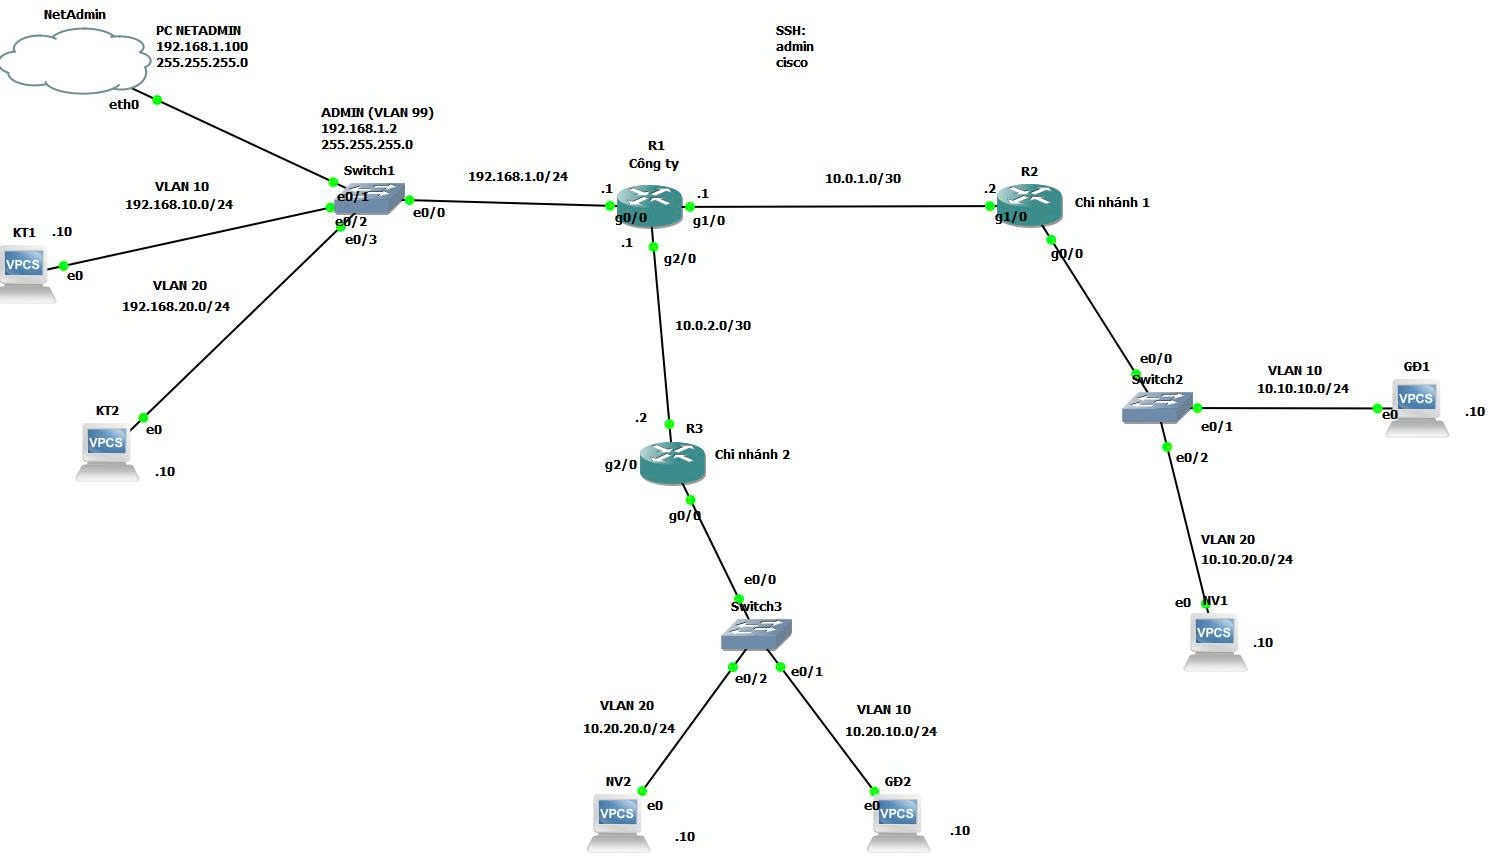
\includegraphics[width=0.7\textwidth]{image/so_do_logic.jpg}
        % 

        \caption{Sơ đồ logic} % Chú thích hình ảnh
        \label{fig:sodo_chen_anh} % Đánh dấu để tham chiếu 
    \end{figure}
    
\subsection{Thông tin IP/VLAN :}

        \label{tab:vlan_allocation}
        \begin{tabular}{|>{\centering\arraybackslash}p{0.5cm} || >{\centering\arraybackslash}p{2cm} || >{\centering\arraybackslash}p{2.5cm} || >{\centering\arraybackslash}p{3cm} || >{\centering\arraybackslash}p{4cm} |}
            \hhline{|=|=|=|=|=|}
            \textbf{No} & \textbf{Khu vực} & \textbf{VLAN Name/Label} & \textbf{Subnet/IP} & \textbf{Mô tả/Ghi chú} \\
            \hhline{|=|=|=|=|=|}
            1 & Công ty (HQ) & VLAN 10 & 192.168.10.0/24 & Phòng kỹ thuật 1 \\
            \hhline{||-||-||-||-||-||} % Chỉ kẻ ngang đơn ở giữa các dòng data
            2 & Công ty (HQ) & VLAN 20 & 192.168.20.0/24 & Phòng kỹ thuật 2 \\
            \hhline{||-||-||-||-||-||}
            3 & Công ty (HQ) & VLAN 99 & 192.168.1.2 & Phòng Network Admin \\
            \hhline{|=|=|=|=|=|} % Đường kẻ đôi ngăn cách khu vực
            4 & Chi nhánh 1 & VLAN 10 & 10.10.10.0/24 & Phòng giám đốc 1 \\
            \hhline{||-||-||-||-||-||}
            5 & Chi nhánh 1 & VLAN 20 & 10.10.20.0/24 & Phòng nhân viên 1 \\
            \hhline{|=|=|=|=|=|}
            6 & Chi nhánh 2 & VLAN 10 & 10.20.10.0/24 & Phòng giám đốc 2 \\
            \hhline{|=|=|=|=|=|}
            7 & Chi nhánh 2 & VLAN 20 & 10.20.10.0/24 & Phòng nhân viên 2 \\
            \hhline{|=|=|=|=|=|}
            8 & WAN Link 1 & R1-R2 Link & 10.0.1.0/30 & Kết nối Công ty - Chi nhánh 1 \\
            \hhline{|=|=|=|=|=|}
            9 & WAN Link 2 & R1-R3 Link & 10.0.2.0/30 & Kết nối Công ty - Chi nhánh 2 \\
            \hhline{|=|=|=|=|=|}
        \end{tabular}

\subsection{Thông tin IP Router và Thiết bị chính :}

% Bắt đầu môi trường bảng
\begin{table}[H]
    \centering 
    
    \label{tab:interface_config}
    
    % Kích thước bảng này khá rộng, nếu bị tràn lề hãy bỏ comment dòng \resizebox bên dưới và dấu } ở cuối
    % \resizebox{\textwidth}{!}{
    
    \begin{tabular}{|>{\centering\arraybackslash}p{0.5cm} || >{\centering\arraybackslash}p{2.5cm} || >{\centering\arraybackslash}p{2cm} || >{\centering\arraybackslash}p{2.8cm} || >{\centering\arraybackslash}p{3cm} || >{\centering\arraybackslash}p{3.5cm} |}
        \hhline{|=|=|=|=|=|=|}
        \textbf{No} & \textbf{Tên thiết bị} & \textbf{Interface} & \textbf{IP Address} & \textbf{Subnet Mask} & \textbf{Ghi chú} \\
        \hhline{|=|=|=|=|=|=|}
        
        % Dòng 1
        1 & PC NETADMIN & eth0 & 192.168.1.100 & 255.255.255.0 & Nối tới Switch1 \\
        \hhline{||-||-||-||-||-||-||} 
        
        % Dòng 2
        2 & \textbf{R1 (Công ty)} & g0/0 & 192.168.1.1 & 255.255.255.0 & \makecell{Gateway \\ cho mạng LAN HQ} \\
        \hhline{||-||-||-||-||-||-||}
        
        % Dòng 3
        3 & \textbf{R1 (Công ty)} & g1/0 & 10.0.1.1 & 255.255.255.252 & Nối đi R2 \\
        \hhline{||-||-||-||-||-||-||}
        
        % Dòng 4
        4 & \textbf{R1 (Công ty)} & g2/0 & 10.0.2.1 & 255.255.255.252 & Nối đi R3 \\
        \hhline{||-||-||-||-||-||-||}
        
        % Dòng 5
        5 & \textbf{PC-KT1} & eth0 & 192.168.10.10 & 255.255.255.0 & Nối tới Switch1 \\
        \hhline{||-||-||-||-||-||-||}
        
        % Dòng 6
        6 & \textbf{PC-KT2} & eth0 & 192.168.20.10 & 255.255.255.0 & \makecell{Nối tới \\ Switch1} \\
        \hhline{||-||-||-||-||-||-||}

        % Dòng 7
        7 & \textbf{R2 (Chi nhánh 1)} & g1/0 & 10.0.1.2 & 255.255.255.252 & Nối về R1 \\
        \hhline{||-||-||-||-||-||-||}

        % Dòng 8
        8 & \textbf{R2 (Chi nhánh 1)} & g0/0 & 192.168.2.1 & 255.255.255.0 & \makecell{Gateway CN1 \\ Nối tới Switch2} \\
        \hhline{||-||-||-||-||-||-||}

        % Dòng 9
        9 & \textbf{PC-GĐ1} & eth0 & 10.10.10.10 & 255.255.255.0 & Nối tới Switch2 \\
        \hhline{||-||-||-||-||-||-||}

        % Dòng 10
        10 & \textbf{PC-NV1} & eth0 & 10.10.20.10 & 255.255.255.0 & Nối tới Switch2 \\
        \hhline{||-||-||-||-||-||-||}

        % Dòng 11
        11 & \textbf{R3 (Chi nhánh 2)} & g2/0 & 10.0.2.2 & 255.255.255.252 & Nối về R1 \\
        \hhline{||-||-||-||-||-||-||}

        % Dòng 12 (Đã sửa lỗi thiếu xuống dòng ở code cũ)
        12 & \textbf{R3 (Chi nhánh 2)} & g0/0 & 192.168.3.1 & 255.255.255.0 & \makecell{Gateway CN2 \\ Nối tới R1} \\
        \hhline{||-||-||-||-||-||-||}

        % Dòng 13
        13 & \textbf{PC-GĐ2} & eth0 & 10.20.10.10 & 255.255.255.0 & Nối tới Switch3 \\
        \hhline{||-||-||-||-||-||-||}

        % Dòng 14 (Đã sửa số thứ tự từ 13 thành 14)
        14 & \textbf{PC-NV2} & eth0 & 10.20.20.10 & 255.255.255.0 & Nối tới Switch3 \\
        \hhline{|=|=|=|=|=|=|}

    \end{tabular}
    
    % } % Đóng ngoặc resizebox nếu dùng
\end{table}
    
\subsection{ Thông tin kết nối:}

    \label{tab:connection_diagram}
    
    % Cấu trúc cột: Thiết bị nguồn, Cổng nguồn, Thiết bị đích, Cổng đích, Mode/Ghi chú
    % Độ rộng cột đã được căn chỉnh để nội dung không bị quá hẹp hoặc quá rộng
    \begin{tabular}{|>{\centering\arraybackslash}p{2.5cm} || >{\centering\arraybackslash}p{1.5cm} || >{\centering\arraybackslash}p{2.5cm} || >{\centering\arraybackslash}p{1.5cm} || >{\centering\arraybackslash}p{4.5cm} |}
        \hhline{|=|=|=|=|=|}
        \textbf{Thiết bị nguồn} & \textbf{Cổng nguồn} & \textbf{Thiết bị đích} & \textbf{Cổng đích} & \textbf{Mode/Ghi chú} \\
        \hhline{|=|=|=|=|=|}
        
        NetAdmin (Cloud) & eth0 & Switch1 & e0/1 & \makecell{Tự động hoá cấu hình \\ các thiết bị} \\
        \hhline{||-||-||-||-||-||} % Kẻ ngang đơn
        
        Switch1 & e0/0 & R1 (Công ty) & g0/0 & Uplink Router \\
        \hhline{||-||-||-||-||-||}
        
        Switch1 & e0/2 & PC KT1 & e0 & VLAN 10 \\
        \hhline{||-||-||-||-||-||}
        
        Switch1 & e0/3 & PC KT2 & e0 & VLAN 20 \\
        \hhline{|=|=|=|=|=|} % Đường kẻ đôi ngăn cách khu vực
        
        R1 (Công ty) & g1/0 & R2 (Chi nhánh 1) & g1/0 & Link WAN 1 \\
        \hhline{||-||-||-||-||-||}
        
        R1 (Công ty) & g2/0 & R3 (Chi nhánh 2) & g2/0 & Link WAN 2 \\
        \hhline{|=|=|=|=|=|}
        
        R2 (Chi nhánh 1) & g0/0 & Switch2 & e0/0 & Downlink LAN \\
        \hhline{||-||-||-||-||-||}
        
        Switch2 & e0/1 & PC GD1 & e0 & VLAN 10 \\
        \hhline{||-||-||-||-||-||}
        
        Switch2 & e0/2 & PC NV1 & e0 & VLAN 20 \\
        \hhline{|=|=|=|=|=|}
        
        R3 (Chi nhánh 2) & g0/0 & Switch3 & e0/0 & Downlink LAN \\
        \hhline{||-||-||-||-||-||}
        
        Switch3 & e0/1 & PC GD2 & e0 & VLAN 10 \\
        \hhline{||-||-||-||-||-||}
        
        Switch3 & e0/2 & PC NV2 & e0 & VLAN 20 \\
        \hhline{|=|=|=|=|=|}
    \end{tabular}
